\chapter{Transfer orbits} %Last updated 3-2-2015
\label{ch:transorb}
The second part of the thesis problem involves (transfer) orbits around Mars. After the ascent phase of the \ac{MAV}, the vehicle will be inserted into an orbit around Mars. Since it will use its high-thrust second-stage engine to perform the final burn to do this it is required to understand the different possible orbits that can be reached using such high-thrust. Therefore \Cref{sec:highthrustorb} will discuss the different high-thrust orbits. At that time, the orbiter should already be in position to rendezvous with the \ac{MAV}. The orbiter will therefore have to travel from its original (operational science) orbit to the rendezvous orbit around Mars. However, compared to the \ac{MAV}, the orbiter will be using a low-thrust propulsion system. These propulsion systems can be turned on for longer amounts of time to provide a continuous thrust. The low-thrust trajectories are discussed in \Cref{sec:lowthrustorb}. Because low-thrust transfers are relatively new, all available planetocentric reference missions have been flown in the Earth system (\Cref{sec:lowthortrref}). The reference mission for low-thrust missions will be discussed and the most important information will be summarized in \Cref{sec:lowthrustorb} as well. \Cref{sec:orbEoM} describes the models and the general \ac{EoM} required to represent the motion of the orbiter. The thrust history for the orbiter can be constructed using the Q-law. This control law is described in \Cref{sec:qlawnbody}. Finally, the Mars 2022 orbiter initial conditions and constraints will be provided in \Cref{sec:2022_ini_con}.



\section{High thrust}
\label{sec:highthrustorb}
The \ac{MAV} will be using a high-thrust propulsion system in the last phase of the ascent, which is the burn into the target orbit. Basically, the \ac{MAV} will transfer from an elliptical (ascent trajectory) 'orbit' to either a circular or a different elliptical orbit around Mars. This orbit injection burn, as it is often called, was described by the equations presented in \Cref{subsec:asc_coast_burn}. This burn does not however include the plane change that might need to be performed. It should be mentioned that any required inclination change between the \ac{MAV} orbit and the orbit of the Mars 2022 orbiter should be performed by the orbiter because a low Mars orbit inclination change with a high-thrust propulsion system requires significantly more energy and thus propellant than an inclination change performed by the low-thrust propulsion system of the Mars 2022 orbiter at a (much) higher orbit \cite{wakker2010}. 

%Both Hohmann and high-energy transfer orbits could be used by the \ac{MAV} should it be required to transfer from its original (parking) orbit to a different orbit. At this point it is assumed that rendezvous will take place in the injected original (parking) orbit of the \ac{MAV}, but in future mission design these transfer orbits can be used to bring the \ac{MAV} to the higher Mars 2022 orbiter orbit should that be required.

%Two types of high-thrust transfer orbits are high-energy transfer and minimum-energy transfer orbits \cite{noomen2013orbit}. This last transfer method is referred to as a Hohmann transfer \cite{wakker2010} and is the most common transfer orbit. It is a direct transfer method, which means that it will directly transfer an \ac{s/c} from one orbit to the other by travelling less than 360$^{\circ}$ (within one rotation) around the main body. In case of a Hohmann transfer, the \ac{s/c} travels 180$^{\circ}$ around Mars before arriving at the destination orbit. This transfer orbit, from one circular orbit to another circular orbit, is characterized by two propulsive shots, one at the departing orbit and one at the destination orbit as illustrated in \Cref{fig:hohmann_braeunig2013} for a heliocentric case \footnote{Source: \url{http://www.braeunig.us/space/interpl.htm} [Accessed 28 October 2015]}. The elliptic orbit touches both the departing and destination planet orbits. 
%
%\begin{figure}[!ht]
%\centering
%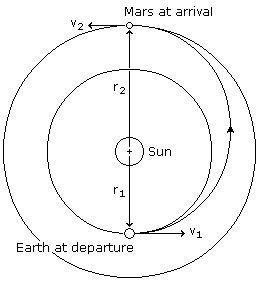
\includegraphics[width=0.3\textwidth]{figures/transfer_orbits/hohmann_braeunig2013.jpg}
%\caption{Graphical representation for Earth-Mars Hohmann transfer burns}
%\label{fig:hohmann_braeunig2013}
%\end{figure}
%
%\nomenclature{$r_{1}$}{Orbital radius of the inner planet\nomunit{m}}
%\nomenclature{$r_{2}$}{Orbital radius of the outer planet\nomunit{m}}
%\nomenclature{$v_{1}$}{Velocity increment required at inner planet (Hohmann)\nomunit{m/s}}
%\nomenclature{$v_{2}$}{Velocity increment required at outer planet (Hohmann)\nomunit{m/s}}
%
%A Homann transfer orbit, in itself, could also be a desired elliptical orbit, in which case only the first burn will have to take place. The process of reaching this desired orbit was described by the equations in \Cref{subsec:asc_coast_burn}. For a Hohmann transfer the planets have to be aligned such that the angle between the departing planet at the time of departure and the destination planet at the time of arrival is 180$^{\circ}$ which only happens every so often. To create more opportunities to reach a certain set point in an orbit, as well as faster, high energy transfer orbits can be applied. In \Cref{fig:highenergy_wakker2010} the four different trajectory types for the ordinary two dimensional case are described for a transfer from Earth to a planet further from the Sun (as an example).
%
%\begin{figure}[!ht]
%\centering
%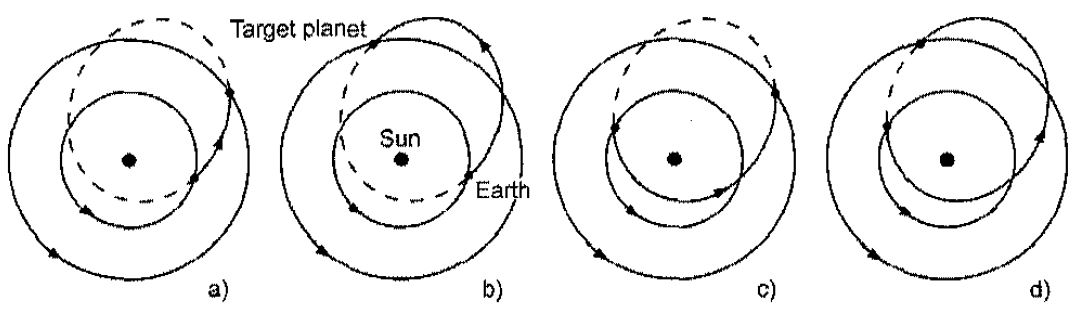
\includegraphics[width=0.5\textwidth]{figures/transfer_orbits/highenergy_wakker2010.jpg}
%\caption{Graphical representation of the four different high energy transfer orbit possibilities based on an arbitrary ellipse crossing both orbits\cite{wakker2010}}
%\label{fig:highenergy_wakker2010}
%\end{figure}
% 
%\nomenclature{$\Delta V$}{Velocity increment\nomunit{m/s}} 
% 
%Figure a) displays the fastest trajectory which is called a type I trajectory. Figure b) represents a so-called type II trajectory where the planet is intercepted at the second crossing of the orbit. Figures c) and d) are similar but for a different starting position of the Earth. Even though the type I trajectory requires more energy, it might be preferred if time is an important factor. A good example of the benefits is provided in \cite{wakker2010}, where it is said that a flight time reduction of 50$\%$ only requires an increase in $\Delta V$ of 19$\%$ but reduces the transferable payload mass by 27$\%$.




\section{Low thrust}
\label{sec:lowthrustorb}
The Mars 2022 orbiter will be using a low-thrust electric propulsion system and will be orbiting the planet to gather scientific data and perform observations. It will also be required to collect the Martian sample from the \ac{MAV} and bring it back to Earth. On a Martian planetocentric level this means that the orbiter will have to travel from its operational science orbit to the lower \ac{MAV} orbit and then back to a higher Martian orbit to escape Mars' gravity well and to reach a suitable Earth return orbit. The low-thrust transfer orbit is described in \Cref{subsec:low_elec_prop} and \Cref{subsec:refrestransorb} describes the reference missions for the Mars 2022 orbiter transfer orbits.

%\subsection{Low-thrust chemical propulsion transfer}
%\label{subsec:low_chem_prop}
%The low-thrust chemical propulsion can be used to get from one orbit to the destination orbit using several impulsive shots. This creates different Hohmann transfer segments and thus takes longer than an ordinary Hohmann transfer. In some cases the \ac{s/c} will have to travel several times around the orbiting body before a certain orbit can be reached as shown in \Cref{fig:lowthrustchem_wertz2009}. In this case the inner circle represents the departing orbit and the outer circle the desired destination orbit that is further away from the orbiting body.   
%
%\begin{figure}[!ht]
%\centering
%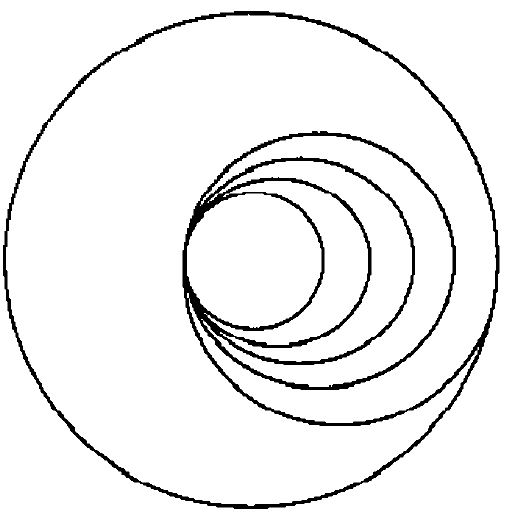
\includegraphics[width=0.2\textwidth]{figures/transfer_orbits/lowthrustchem_wertz2009.jpg}
%\caption{Example low thrust transfer trajectory using Hohmann segments\cite{wertz2009}}
%\label{fig:lowthrustchem_wertz2009}
%\end{figure}



\subsection{Low-thrust electrical propulsion transfer}
\label{subsec:low_elec_prop}
Low-thrust electric propulsion is characterised by a high specific impulse ($I_{sp}$) but very low thrust levels. It is very useful for long-duration missions and these engines can thrust continuously if necessary. This continuous thrusting would result in a spiral orbit as depicted in \Cref{fig:contelec_wertz2009}, however the thrust can also be applied in increments where there are thrusting periods and coasting periods in the transfer orbit. This was for instance done by the Dawn spacecraft in combination with gravity assists (see \Cref{fig:dawntrajectory_wakker2010}).

%\nomenclature{$I_{sp}$}{Specific impulse\nomunit{s}}

\begin{figure}[!ht]
\centering
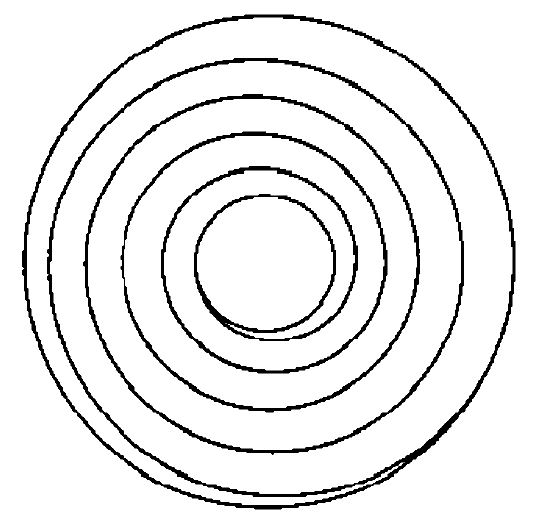
\includegraphics[width=0.3\textwidth]{figures/transfer_orbits/contelec_wertz2009.jpg}
\caption{Example of continuous low-thrust trajectory \cite{wertz2009}.}
\label{fig:contelec_wertz2009}
\end{figure}


\begin{figure}[!ht]
\centering
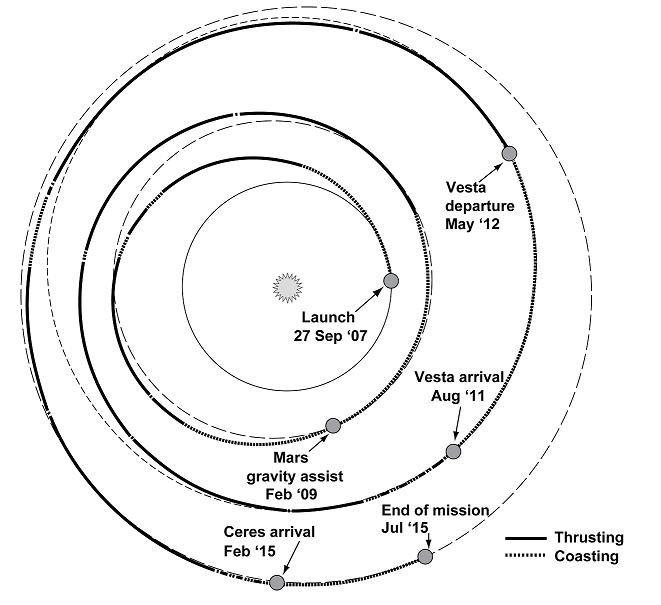
\includegraphics[width=0.4\textwidth]{figures/transfer_orbits/dawntrajectory_wakker2010.jpg}
\caption{Example of a segmented low-thrust interplanetary trajectory: the Dawn transfer \cite{wakker2010}.}
\label{fig:dawntrajectory_wakker2010}
\end{figure}

\subsection{Reference missions}
\label{subsec:refrestransorb}
The Mars 2022 orbiter will be propelled by an \ac{EP} system, thus a spiralling transfer motion can be expected. The reference missions and research mentioned in \Cref{sec:lowthortrref} also used \ac{EP}. Deep Space 1 is considered to be the first modern \ac{s/c} to use \ac{EP} as its main propulsion system used to perform orbital transfer manoeuvres. The engine was a Xenon ion engine. Ever since this mission Xenon engines have become increasingly popular and almost all modern low-thrust missions now use such engines \cite{wakker2010}. These engines are either Hall thrusters or full ion engines. In \Cref{tab:xenon_ref_missions} all flown reference missions that used either of these engines are mentioned and their engine characteristics are specified. This table also includes interplanetary missions.

\begin{table}[!ht]
\begin{center}
\caption{Flown low-thrust missions using Xenon engines and their characteristics (provided per thruster).}
\label{tab:xenon_ref_missions}
\begin{tabular}{|l|l|l|p{1.5cm}|p{1.5cm}|p{2cm}|l|l|l|}
\hline 
\textbf{Year} 		& \textbf{Mission/\ac{s/c}} & \textbf{Engine} & \textbf{Thrusters} & \textbf{Thrusters active at once} & \textbf{Engine power [kW]} & $\mathbf{I_{sp}}$ \textbf{[s]} & \textbf{Thrust [mN]} & \textbf{Ref.} \\ \hline \hline
1998 &  Deep Space 1 & Ion & 1 & 1 & 2.5 (max) & 3120 & 92.4 & \cite{polk1999validation,wakker2010,martinez1998spacecraft}\\ \hline
2001 & Artemis & Ion & 4 & 1 & 0.57 & 3370 & 15 $\pm$0.9\% & \cite{killinger2003artemis} \tablefootnote{Artemis mission update: \url{http://m.esa.int/Our_Activities/Telecommunications_Integrated_Applications/Artemis_finally_reaches_operational_orbit} [Accessed 18 October 2015]}\\ \hline
2003 &  Hayabusa & Ion & 4 & 3 & 0.38 & 3160 & 8 & \cite{wakker2010}  \\ \hline
2003 &  SMART-1 & Hall & 1 & 1 & 1.19 & 1631 & 68 &  \cite{wakker2010} \\ \hline
2007 &  Dawn & Ion & 3 & 1 & 2.6 & 3058 & 92 & \cite{wakker2010}  \\ \hline
2010 & AEHF(-1) & Hall & 4 & 2 & 4.5 & 2020 & 267 & Updates \tablefootnote{AEHF-1 mission update: \url{http://spaceflightnow.com/atlas/av019/111009.html} [Accessed 18 October 2015]} $^{,}$ \tablefootnote{Online catalogue Aerojet Rocketdyne: \url{https://www.rocket.com/propulsion-systems/electric-propulsion} [Accessed 25 November 2015]}\\ \hline
2015 & Boeing 702SP & Ion & 4 & 1\tablefootnote{Assumed 1 provided that the maximum available power is 9 kW, or 2 if no other system is active, which is less likely} & 4.5 & 3500 & 165 & \cite{esa2015all,schaeff2014low} \tablefootnote{Boeing company: \url{http://www.boeing.com/space/boeing-satellite-family/index.page} [Accessed 18 October 2015]} \\ \hline

\end{tabular}
\end{center}
\end{table}



%It can be seen that the Xenon ion engines have a much higher specific impulse than the Xenon Hall engines. \\

There are already many different programs available that can simulate low-thrust trajectories. In three of the mentioned papers in \Cref{subsec:lowrefres} the different used methods, dynamic equations and \ac{EoM} are described. \cite{geffroy1997optimal} and \cite{kluever1998direct} used the classical non-singular equinoctial orbital elements, instead of the Kepler elements, and their corresponding \ac{EoM} to determine the orbit trajectories, whereas \cite{whiffen2006mystic} describes a method of using Cartesian coordinates and the corresponding \ac{EoM}. These reference methods can be used in the next section to set-up the  dynamic model and corresponding \ac{EoM} for the thesis problem.


\section{Dynamic model and Equations of Motion}
\label{sec:orbEoM}
For the simulation of the orbiter motion it is important to have an accurate representation of reality. However, it should also still be possible to find a solution to the problem, which means that the model should also not be too complex. Most of the low-thrust model will be based on the work of Gebbett \cite{gebbett2014multi} and thus the same assumptions will be made and equations will be used. The dynamic model is described in \Cref{subsec:dynmod_orb} and the corresponding \ac{EoM} are provided in \Cref{subsec:eom_orb}.

%
%This part of the thesis will be based on Warren's work and will thus be using his approach.\\

\subsection{Dynamic model and initial assumptions}
\label{subsec:dynmod_orb}
The motion of an \ac{s/c} around a body can be described by Kepler elements (\Cref{fig:kepler_noomen2013basic_akcasu2013}) where $a$ is the semi-major axis, $e$ is the eccentricity, $i$ the orbit inclination, $\omega$ the argument of periapsis, $\Omega$ the right ascension of the ascending node and $\theta$ the true anomaly. In a normal stable orbit all these elements except for $\theta$ are constant. The elements are in this case described in an inertial planet-centred reference frame.

\begin{figure}[!ht]
\centering
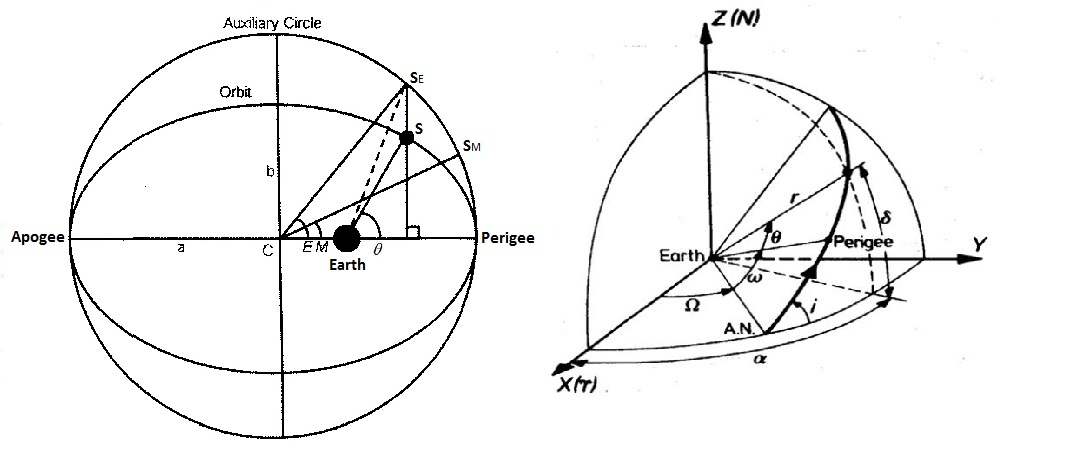
\includegraphics[width=1.0\textwidth]{figures/reference_frames/kepler_noomen2013basic_akcasu2013.jpg}
\caption{Definition of the Kepler elements in 2D (left) and 3D (right) \cite{noomen2013basic,akcasu2013}.}
\label{fig:kepler_noomen2013basic_akcasu2013}
\end{figure}

A stable orbit can however be disturbed which will cause the orbital elements to change and thus result in a different orbit. These disturbances are called orbital perturbations. During the orbital change of the Mars 2022 orbiter, the low-thrust propulsion system will cause a perturbation to change from one orbit to the other, however there are also other effects that can cause the orbit to change. The most important perturbations that were taken into account by \cite{gebbett2014multi} and that are meaningful to take into account in an orbit around Mars are the $J_{2}$ gravitational (flattening) effect, and the third-body perturbation caused by the Sun. Both effects will be discussed in the next section. Another element that is taken into account in the low-thrust orbital model is the shadowing effect of the planet. The orbiter will be using a propulsion technology called \ac{SEP} which requires such a great amount of power that it can only be used when the \ac{s/c} is in direct sunlight. Therefore the propulsion system cannot be used during eclipse, which has to be taken into account when designing the propulsion scheme for the low-thrust orbit trajectory. More information on the application of the shadowing effect in the simulation tool can be found in \cite{gebbett2014multi}.
 

\subsection{Corresponding \ac{EoM} and initial assumptions}
\label{subsec:eom_orb}
To model the changes in the orbital elements as a result of the thrust and the different perturbations, Gauss' form of the Lagrange's planetary equations as shown by \Cref{eq:gauss} are recommended \cite{wakker2010,gebbett2014multi,petropoulos2005refinements}. Here $f_{S}$, $f_{N}$ and $f_{W}$ are defined as in \Cref{fig:sc_acc_wakker2010} and $p$ is the semi-latus rectum defined as $a\left(1-e^{2}\right)$.

\nomenclature[R8]{$p$}{Semi-latus rectum \nomunit{m}}
\nomenclature[R2]{$f_{S}$}{Radial perturbing acceleration \nomunit{m/s$^{2}$}}
\nomenclature[R2]{$f_{N}$}{Perturbing acceleration perpendicular to the radius vector \nomunit{m/s$^{2}$}}
\nomenclature[R2]{$f_{W}$}{Perturbing acceleration perpendicular to the orbital plane \nomunit{m/s$^{2}$}}

\begin{equation} \label{eq:gauss}
\begin{split}
\dfrac{da}{dt}&=2\dfrac{a^{2}}{\sqrt{\mu_{M}p}}\left[e\sin\left(\theta\right)f_{S}+\dfrac{p}{r}f_{N}\right]\\
\dfrac{de}{dt}&=\dfrac{1}{\sqrt{\mu_{M}p}}\left[p\sin\left(\theta\right)f_{S}+\left(\left(p+r\right)\cos\left(\theta\right)+re\right)f_{N}\right]\\
\dfrac{di}{dt}&=\dfrac{r}{\sqrt{\mu_{M}p}}\cos\left(\theta+\omega\right)f_{W}\\
\dfrac{d\omega}{dt}&=\dfrac{1}{e \sqrt{\mu_{M}p}}\left[-p\cos\left(\theta\right)f_{S}+\left(p+r\right)\sin\left(\theta\right)f_{N}\right]-\dfrac{r\sin\left(\theta+\omega\right)\cos\left(i\right)}{\sqrt{\mu_{M}p}\sin\left(i\right)}f_{W}\\
\dfrac{d\Omega}{dt}&=\dfrac{r}{\sqrt{\mu_{M}p}\sin\left(i\right)}\sin\left(\theta+\omega\right)f_{W}\\
\dfrac{d\theta}{dt}&=\dfrac{\sqrt{\mu_{M}p}}{r^{s}}+\dfrac{1}{e \sqrt{\mu_{M}p}}\left[p\cos\left(\theta\right)f_{S}-\left(p+r\right)\sin\left(\theta\right)f_{N}\right]\\
\end{split}
\end{equation}


\begin{figure}[!ht]
\centering
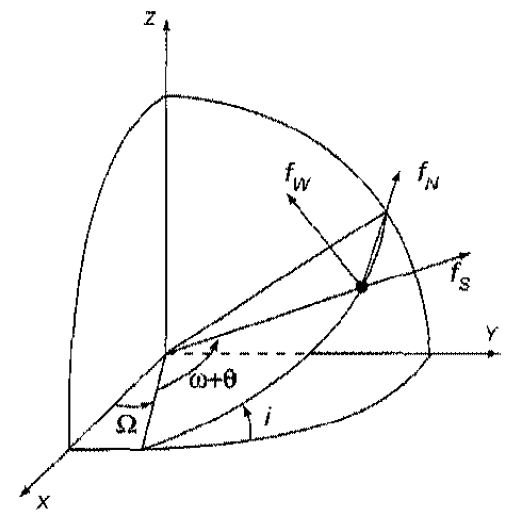
\includegraphics[width=0.4\textwidth]{figures/transfer_orbits/sc_acc_wakker2010.jpg}
\caption{Definition of the perturbing accelerations \cite{wakker2010}.}
\label{fig:sc_acc_wakker2010}
\end{figure}

However, it is clear that for $e=0$ and/or $i=0^{\circ}$ or $180^{\circ}$ this set of equations results in singularities. Therefore a slightly modified set of elements is used to eliminate these singularities. In \cite{gebbett2014multi} the \ac{MEE} were deemed most suited based on the survey performed in \citep{hintz2008survey} because this set is non-singular. The definition of the six elements is provided in \Cref{eq:MEE}, where the semi-latus rectum is still the same as defined before but now directly used. More information on the \ac{MEE} was provided in \Cref{ch:reftrans}. 

%\begin{equation} \label{eq:MEE}
%\begin{split}
%p&=a\left(1-e^{2}\right)\\
%f&=e\cos\left(\omega+I\Omega\right)\\
%g&=e\sin\left(\omega+I\Omega\right)\\
%h&=\tan^{I}\left(\dfrac{i}{2}\right)\cos\left(\Omega\right)\\
%k&=\tan^{I}\left(\dfrac{i}{2}\right)\sin\left(\Omega\right)\\
%L&=\omega+\theta+I\Omega\\
%\end{split}
%\end{equation}


\begin{align} \label{eq:MEE}
\begin{split} 
p&=a\left(1-e^{2}\right)\\
f&=e\cos\left(\omega+I\Omega\right)\\
g&=e\sin\left(\omega+I\Omega\right)
\end{split} 
&
\begin{split}
h&=\tan^{I}\left(\dfrac{i}{2}\right)\cos\left(\Omega\right)\\
k&=\tan^{I}\left(\dfrac{i}{2}\right)\sin\left(\Omega\right)\\
L&=\omega+\theta+I\Omega
\end{split}
\end{align}

\nomenclature[R5]{$L$}{True longitude \nomunit{rad}}


In \Cref{eq:MEE} $I$ is the retrograde factor and has a value of +1 for posigrade orbits and -1 for retrograde orbits. This is done to avoid singularities when $i=180^{\circ}$ and thus making the set non-singular.

\nomenclature[R5]{$I$}{Retrograde factor \nomunit{-}}

The corresponding differential equations are also provided in \cite{hintz2008survey} and corrected by \cite{gebbett2014multi}. These corrected equations are shown in \Cref{eq:eom_mee} where $s^{2}=1+h^{2}+k^{2}$ and $w=p/r=1+f\cos\left(L\right)+g\sin\left(L\right)$. These equations are used to propagate the orbit.

\begin{equation} \label{eq:eom_mee}
\begin{split}
\dfrac{dp}{dt}&=\dfrac{2p}{w}\sqrt{\dfrac{p}{\mu_{M}}}f_{N}\\
\dfrac{df}{dt}&=\sqrt{\dfrac{p}{\mu_{M}}}\left[\sin\left(L\right)f_{S}+\left(\left(w+1\right)\cos\left(L\right)+f\right)\dfrac{f_{N}}{w}-\left(h\sin\left(L\right)-k\cos\left(L\right)\right)g\dfrac{f_{W}}{w}\right]\\
\dfrac{dg}{dt}&=\sqrt{\dfrac{p}{\mu_{M}}}\left[-\cos\left(L\right)f_{S}+\left(\left(w+1\right)\cos\left(L\right)+g\right)\dfrac{f_{N}}{w}+\left(h\sin\left(L\right)-k\cos\left(L\right)\right)f\dfrac{f_{W}}{w}\right]\\
\dfrac{dh}{dt}&=\sqrt{\dfrac{p}{\mu_{M}}}\dfrac{s^{2}f_{W}}{2w}\cos\left(L\right)\\
\dfrac{dk}{dt}&=\sqrt{\dfrac{p}{\mu_{M}}}\dfrac{s^{2}f_{W}}{2w}\sin\left(L\right)\\
\dfrac{dL}{dt}&=\sqrt{\mu_{M}p}\left(\dfrac{w}{p}\right)^{2}+\dfrac{1}{w}\sqrt{\dfrac{p}{\mu_{M}}}\left(h\sin\left(L\right)=k\cos\left(L\right)\right)f_{W}\\
\end{split}
\end{equation}
%&=\\

When it comes to the other perturbations, these can simply be added as an extra effect in any of the three perturbation acceleration directions. $J_{2}$ on Mars has a value of 1960.45$\cdot$ 10$^{-6}$ \cite{williams2015}. The general equations for gravitational perturbations in normal Kepler elements are discussed in \cite{noomen2011kepler}, however in this case, the same equations are needed for the \ac{MEE}. Fortunately, these are provided by \cite{kechichian2000minimum} and are given in \Cref{eq:j2}. Here $s$ is again defined as for \Cref{eq:eom_mee}.

\begin{equation} \label{eq:j2}
\begin{split}
f_{S,J_{2}}&=-\dfrac{3\mu_{M}J_{2}R_{M}^{2}}{2r^{4}}\left(1-12\dfrac{\left(h\sin\left(L\right)-k\cos\left(L\right)\right)^{2}}{s^{4}}\right)\\
f_{N,J_{2}}&=-\dfrac{12\mu_{M}J_{2}R_{M}^{2}}{r^{4}}\left(\dfrac{\left(h\sin\left(L\right)-k\cos\left(L\right)\right)\left(h\cos\left(L\right)+k\sin\left(L\right)\right)}{s^{4}}\right)\\
f_{W,J_{2}}&=-\dfrac{6\mu_{M}J_{2}R_{M}^{2}}{r^{4}}\left(\dfrac{\left(h\sin\left(L\right)-k\cos\left(L\right)\right)\left(1-h^{2}-k^{2}\right)}{s^{4}}\right)\\
\end{split}
\end{equation}
%&=\\

%implement equations for J2\\
%1960.45$\cdot$ 10$^{-6}$ \cite{williams2015}

The perturbing acceleration caused by a third body are important to take into account if the third body has a high mass compared to the primary (orbiting) body. Mars has two natural satellites: Phobos and Deimos. However, the mass of these two satellites is relatively small compared to that of Mars \cite{williams2015}. The gravitational acceleration of Phobos acting on an orbiting \ac{s/c} is on the order of 10$^{-8}$ (compared to the accelerations caused by the J2-effect, which is in the order of 10$^{-3}$). Thus it is assumed that the Martian moons do not have to be taken into account in the third-body perturbations, however should this decision change, they can always be added in the future. Also, the orbit of Mars 2022 will be different from that of the two moons, which will reduce the effects even more. The Sun however is a body that will be taken into account, because the gravitational accelerations are in the order of 10$^{-7}$ and are almost always present. In \cite{gebbett2014multi} a method by Battin \cite{battin1999introduction} is used to determine the accelerations caused by the third body, which in this case is the Sun. Battin's function is described in \Cref{eq:battin} where $\mathbf{r}$ is the position vector of the orbiter with respect to Mars and $\mathbf{r_{MS}}$ is the position vector of the Sun with respect to Mars.

\nomenclature[Ra0]{$r_{MS}$}{Distance between Mars and the Sun \nomunit{m}}

\begin{equation} \label{eq:battin}
f\left(q\right)=q\left[\dfrac{3+3q+q^{2}}{1+\left(1+q\right)^{\frac{3}{2}}}\right] \qquad \text{where} \qquad q=\dfrac{\mathbf{r} \mathbf{\cdot}\left(\mathbf{r}-2\mathbf{r_{MS}}\right)}{\mathbf{r_{MS}\cdot r_{MS}}}
\end{equation}

The third-body acceleration can then be described by \Cref{eq:third_b_per}. Please note that these accelerations are described in the inertial Mars-centred frame in Cartesian coordinates and will thus have to be transformed to the \ac{s/c} centred orbital frame (\Cref{fig:sc_acc_wakker2010}) to be added to the other accelerations that are acting on the orbiter. This transformation was described in \Cref{ch:reftrans}.

\begin{equation} \label{eq:third_b_per}
\mathbf{a}_{S}=-\dfrac{\mu_{S}}{\left(\mathbf{r}-\mathbf{r_{MS}}\right)^{3}}\left(\mathbf{r}+f\left(q\right)\mathbf{r_{MS}}\right)
\end{equation}

%\nomenclature{$\mu_{S}$}{Standard gravitational parameter of the Sun \nomunit{m$^{3}$/s$^{2}$}}

%and implement equations for third body\\

Here the standard gravitational parameter for the perturbing body, in this case the Sun, is used. For a given position of the celestial bodies and the orbiting \ac{s/c} the most important perturbations can now be computed. 


\section{Q-law}  %and the N-body problem
\label{sec:qlawnbody}
During the transfer of the orbiter, the low-thrust engine will be used to perform the orbital changes. However, unlike high-thrust engines, low-thrust engines can be active for a long period of time. They can also be turned off and on again. Determining the time that the engines have to be active and in which direction the thrust has to be pointed can be very difficult and time consuming. This is why, at \ac{JPL} back in 2003, Petropoulos developed a feedback control law called Q-law \cite{petropoulos2003simple}, which can very accurately provide a good representation of the thrusting behaviour required to get from a starting orbit to a target orbit. The specific point in that orbit $\theta$ can not be pre-set. In the years following, the Q-law was refined (\cite{petropoulos2004low,petropoulos2005refinements}) and the latest version of the fundamental function Q is presented in \Cref{eq:Q}.

\begin{equation} \label{eq:Q}
Q=\left(1+W_{P}P\right)\displaystyle\sum_{\oe}W_{\oe}S_{\oe}\left[\dfrac{d\left(\oe,\oe_{T}\right)}{\tilde{\dot{\oe}}_{xx}}\right]^{2},\qquad  \text{for} \qquad \oe=a,e,i,\omega,\Omega
\end{equation}

\nomenclature[R9]{$Q$}{Q-law function in Kepler elements \nomunit{s$^{2}$}}
\nomenclature[S]{$\oe$}{Orbital element \nomunit{-}}
\nomenclature[Ra4]{$W_{\oe}$}{Orbital element weight \nomunit{-}}
\nomenclature[Ra3]{$W_{P}$}{Penalty function weight \nomunit{-}}


Here $W_{P}$ and $W_{\oe}$ are weights which have a scalar value equal to or greater than 0. $P$ is a penalty function depending on the problem, but in \cite{petropoulos2005refinements} it was used to define a minimum periapsis radius which the orbit had to satisfy. This function is defined in \Cref{eq:P}. $S_{\oe}$ is a scalar function as defined by \Cref{eq:S} and $d\left(\oe,\oe_{T}\right)$ is a distance function (see \Cref{eq:doeoet}) where the subscript $T$ stands for target. Finally, $\tilde{\dot{\oe}}_{xx}$ represents the maximum rate of change of the orbital elements over the thrust direction and true anomaly as defined by \Cref{eq:crazy_oe}. 

\begin{equation} \label{eq:P}
P=exp\left[k\left(1-\dfrac{r_{p}}{r_{p,min}}\right)\right]
\end{equation}

Here $k$ is a scalar that can be adjusted if required. For instance, if at the end of the propagation it turns out that during the propagation the orbit went 2 km below the allowed minimum perigee radius and it is preferred to only go 1 km below the allowed minimum perigee radius, then the value for $k$ should be increased. This is typically done by trial and error.

\nomenclature[R5]{$k$}{Penalty function adjustable scalar \nomunit{-}}

\begin{equation}\label{eq:S}
S_{\oe}=\begin{cases}
\left[1+\left(\dfrac{a-a_{T}}{ma_{T}}\right)^{n}\right]^{\dfrac{1}{r}}, & \text{for } \oe=a\\
1, & \text{for } \oe=e,i,\omega,\Omega
\end{cases}
\end{equation}

In \Cref{eq:S} the nominal values for $m$, $n$ and $r$ are respectively 3, 4 and 2. 


\begin{equation}\label{eq:doeoet}
d\left(\oe,\oe_{T}\right)=\begin{cases}
\oe-\oe_{T}, & \text{for } \oe =a,e,i\\
\arccos\left[\cos\left(\oe-\oe_{T}\right)\right], & \text{for } \oe=\omega,\Omega \quad \text{where} \quad \cos\left(\oe-\oe_{T}\right)\in \left[0,\pi\right]
\end{cases}
\end{equation}

%Here $\cos\left(\oe-\oe_{T}\right)\in \left[0,\pi\right]$.

\begin{equation}\label{eq:crazy_oe}
\tilde{\dot{\oe}}_{xx}=\begin{cases}
\dot{\oe}_{xx}=\displaystyle\max_{\alpha,\beta,\theta}, & \text{for } \oe =a,e,i,\Omega\\
\left(\dot{\omega}_{xxi}+b\dot{\omega}_{xxo}\right)/\left(1+b\right), & \text{for } \oe=\Omega
\end{cases}
\end{equation}

Here $\dot{\oe}$ are provided by \Cref{eq:gauss}, $\alpha \in [-\pi,\pi]$ is the in-plane thrust angle and $\beta \in [-\dfrac{\pi}{2},\dfrac{\pi}{2}]$ is the out-of-plane thrust angle \cite{gebbett2014multi}. The subscript x means that it is a maximum. In this case two x's are used because first the maximum is taken using a combination of $\alpha$ and $\beta$ resulting in $\dot{\oe}_{x}$ and then the maximum is taken using $\theta$ thus resulting in the notation $\dot{\oe}_{xx}$. Also, $b$ is a non-negative constant with a nominal value of 0.01 and both $\dot{\omega}_{xxi}$ and $\dot{\omega}_{xxo}$ are defined in \Cref{eq:omega_dot}.

\nomenclature[G]{$\alpha$}{In-plane thrust angle \nomunit{rad}}
\nomenclature[G]{$\beta$}{Out-of-plane thrust angle \nomunit{rad}}

\begin{equation} \label{eq:omega_dot}
\begin{split}
\dot{\omega}_{xxi} &=\displaystyle\max_{\alpha,\theta}\left(\dot{\oe}|_{\beta=0}\right)\\
\dot{\omega}_{xxo} &=\displaystyle\max_{\theta}\left(\dot{\oe}|_{\beta=\pi/2}\right)
\end{split}
\end{equation}

Now using \Cref{eq:fthrust}, the accelerations in \Cref{eq:eom_mee} can be written such that $Q$ is not a function of $\alpha$, $\beta$ and $\theta$ as described in \cite{petropoulos2005refinements}.

\begin{equation} \label{eq:fthrust}
\begin{split}
f_{S}&=f_{Thrust}\cos\left(\beta\right)\sin\left(\alpha\right)\\
f_{N}&=f_{Thrust}\cos\left(\beta\right)\cos\left(\alpha\right)\\
f_{W}&=f_{Thrust}\sin\left(\beta\right)
\end{split}
\end{equation}

\nomenclature[R2]{$f_{Thrust}$}{Total thrust acceleration \nomunit{m/s$^{2}$}}

Q is zero at the target orbit and positive elsewhere. The greater the value of Q the further away the \ac{s/c} is from the target orbit. The idea is to reduce Q to zero as soon as possible. Therefore at every time step, the largest reduction of Q is required. This can be computed through \Cref{eq:qdot}. Here the subscript n denotes that it is a minimum.

\begin{equation} \label{eq:qdot}
\begin{split}
\dfrac{dQ}{dt}=\dot{Q}&=\displaystyle\sum_{\oe}\dfrac{\delta Q}{\delta \oe}\dot{\oe}\\
\dot{Q}_{n} &= \displaystyle\min_{\alpha,\beta}\dot{Q}
\end{split}
\end{equation}

From this it can be determined in which direction the thrust has to be directed. The next step is to determine whether it is useful to provide this thrust at this instance or not. This is done through the so-called effectivity. The absolute and relative effectivity are defined as in \Cref{eq:effect}.

% where $\dot{Q}_{nn}$ and $\dot{Q}_{nx}$ are given by \Cref{eq:minmaxQdotn}

%\begin{equation} \label{eq:effect}
%\begin{split}
%\eta_{a}&=\dfrac{\dot{Q}_{n}}{\dot{Q}_{nn}}\\
%\eta_{r} &= \dfrac{\dot{Q}_{n}-\dot{Q}_{nx}}{\dot{Q}_{nn}-\dot{Q}_{nx}}
%\end{split}
%\end{equation}

\nomenclature[G3]{$\eta_{a}$}{Absolute effectivity \nomunit{-}}
\nomenclature[G3]{$\eta_{r}$}{Relative effectivity \nomunit{-}}

%\begin{equation} \label{eq:minmaxQdotn}
%\begin{split}
%\dot{Q}_{nn}&=\displaystyle\min_{\theta}\dot{Q}_{n}\\
%\dot{Q}_{nx} &= \displaystyle\max_{\theta}\dot{Q}_{n}
%\end{split}
%\end{equation}

\begin{align} \label{eq:effect}
\begin{split} 
\eta_{a}&=\dfrac{\dot{Q}_{n}}{\dot{Q}_{nn}}\\
\eta_{r} &= \dfrac{\dot{Q}_{n}-\dot{Q}_{nx}}{\dot{Q}_{nn}-\dot{Q}_{nx}}
\end{split} 
&
\begin{split}
where \quad \dot{Q}_{nn}&=\displaystyle\min_{\theta}\dot{Q}_{n}\\
where \quad \dot{Q}_{nx} &= \displaystyle\max_{\theta}\dot{Q}_{n}
\end{split}
\end{align}

\nomenclature[G3]{$\eta_{cut}$}{Cut effectivity  \nomunit{-}}

It is up to the user to determine which of the two effectivities to use, because it is problem dependent. But both values will have to be higher than a certain cut-off value $\eta_{cut}$ for the control law to accept it as a point where thrust has to be applied. If the effectivity is lower than this $\eta_{cut}$ it means that no thrust will be applied and the \ac{s/c} is thus in a coasting phase. According to Petropoulos it is better to use the relative (rather than absolute) effectivity for near-circular orbits, which is based on his experience.\\
The equation for the Q-law itself is used to determine the direction in which thrust has to be applied and the Q-law effectivity determines whether this thrust should be applied or not. This results in a thrust which is incorporated in the orbit propagation. However, in its current form, singularities can occur, which is why \cite{gebbett2014multi} wrote the Q-law in \ac{MEE} using the Gauss' equations provided in \Cref{eq:eom_mee}.  This form (described by \cite{gebbett2014multi}) will also be used in the thesis problem to avoid any singularities and to be able to optimise for every kind of orbit.\\

The simplified form of the Q-law using \ac{MEE} is provided by \Cref{eq:Qmee}\cite{gebbett2014multi}. This formulation is similar to the original Q-law formulation that was introduced in 2003 \cite{petropoulos2003simple}.


\begin{equation} \label{eq:Qmee}
Q_{MEE}=\displaystyle\sum_{\xi}W_{\xi}\left[\dfrac{\xi-\xi_{t}}{\dot{\xi}_{x}}\right]^{2},\qquad  for \qquad \xi=p,f,g,h,k
\end{equation}

\nomenclature[G5]{$\xi$}{Non-singular orbital element \nomunit{-}}
\nomenclature[R9]{$Q_{MEE}$}{Non-singular Q-law \nomunit{s$^{2}$}}

%\left(1+W_{P}P\right)

Again $W_{\xi}$ are  weights with a scalar value equal to or greater than 0 and $\xi$ depicts the \ac{MEE}. Also, since only one maximum is taken (only the maximum with respect to $L$) the notation for $\dot{\xi}_{x}$ has one $x$ in the subscript. In this case Gebbett found that it is more computationally efficient to use the expressions for the accelerations in the different directions directly instead of using the two thrust angles. Therefore, the expressions for $\dot{\xi}_{x}$ are found through the \ac{EoM} given by \Cref{eq:eom_mee} and applying \Cref{eq:max_L}.

\begin{equation} \label{eq:max_L}
\dot{\xi}_{x}=\displaystyle\max_{L}\left(\dot{\xi}\right) \qquad for \qquad \xi=p,f,g,h,k 
\end{equation}

For $\dot{p}_{x}$, $\dot{h}_{x}$ and $\dot{k}_{x}$ the analytical expressions for the critical points can be found for which $L$ is maximum. The value for $\dot{p_{x}}$, $\dot{h_{x}}$ and $\dot{k_{x}}$ is then the maximum of both critical values resulting from the equations mentioned in \Cref{eq:crit_phk} \cite{gebbett2014multi}.

\begin{equation} \label{eq:crit_phk}
\begin{split}
\dot{p}_{x}&=\max\left(\dot{p}_{cr}\right), \qquad \dot{p}_{cr}=\dfrac{2p}{1\pm \dfrac{f}{\sqrt{\dfrac{g^{2}}{f^{2}}+1}}\pm\dfrac{g}{f\sqrt{\dfrac{g^{2}}{f^{2}}+1}}}\sqrt{\dfrac{p}{\mu_{M}}f_{Thrust}}\\
\dot{h}_{x}&=\max\left(\dot{h}_{cr}\right), \qquad \dot{h}_{cr}=\dfrac{\pm \sqrt{1-g^{2}}}{1\pm f\sqrt{1-g^{2}}-g^{2}}\sqrt{\dfrac{p}{\mu_{M}}\dfrac{s^{2}}{2}}f_{Thrust}\\
\dot{k}_{x}&=\max\left(\dot{k}_{cr}\right), \qquad \dot{k}_{cr}=\dfrac{\pm \sqrt{1-f^{2}}}{1\pm g\sqrt{1-f^{2}}-f^{2}}\sqrt{\dfrac{p}{\mu_{M}}\dfrac{s^{2}}{2}}f_{Thrust}\\
\end{split}
\end{equation}

Because $\dot{f}$ and $\dot{g}$ are a function of all the three acceleration directions, a direct analytical solution was deemed impossible to find by \cite{gebbett2014multi}. Therefore the functions have to be evaluated numerically for $L$ to determine the critical values for the three different accelerations. The equations for $\dot{f}$ and $\dot{g}$ (\Cref{eq:eom_mee}) can be slightly rewritten to single out the different accelerations as shown in \Cref{eq:crit_fg}. Here $H(L)$, $J(L)$ and $K(L)$ are simply the rewritten parts of the original expression and are shown in \Cref{eq:HJK_fg} for both $\dot{f}$ and $\dot{g}$ respectively.

\begin{equation} \label{eq:crit_fg}
\begin{split}
\dot{f}&=H_{f}(L)f_{S}+J_{f}(L)f_{N}+K_{f}(L)f_{W}\\
\dot{g}&=H_{g}(L)f_{S}+J_{g}(L)f_{N}+K_{g}(L)f_{W}\\
\end{split}
\end{equation}



\begin{align} \label{eq:HJK_fg}
\begin{split} 
H_{f}&=\sqrt{\dfrac{p}{\mu_{M}}}\sin\left(L\right)\\
J_{f}&=\sqrt{\dfrac{p}{\mu_{M}}}\dfrac{\left(w+1\right)\cos\left(L\right)+f}{w}\\
K_{f}&=-\sqrt{\dfrac{p}{\mu_{M}}}\dfrac{h\sin\left(L\right)-k\cos\left(L\right)}{w}g
\end{split} 
&
\begin{split}
H_{g}&=-\sqrt{\dfrac{p}{\mu_{M}}}\cos\left(L\right)\\
J_{g}&=\sqrt{\dfrac{p}{\mu_{M}}}\dfrac{\left(w+1\right)\cos\left(L\right)+g}{w}\\
K_{g}&=\sqrt{\dfrac{p}{\mu_{M}}}\dfrac{h\sin\left(L\right)-k\cos\left(L\right)}{w}f
\end{split}
\end{align}



It is mentioned that this method is very slow, but it does result in a robust system that can handle both elliptic and circular orbits. To have a slightly faster evaluation \cite{gebbett2014multi} decided to evaluate $\dot{f}_{x}$ and $\dot{g}_{x}$ only once every revolution because the orbital elements do not show a significant difference in that one revolution. This is only an approximation but in \Cref{eq:Qmee} the weights can be used to make the contribution of both $\dot{f}_{x}$ and $\dot{g}_{x}$ less important and have a lower influence on the solution. $Q_{MEE}$ is again zero at the target orbit and positive elsewhere. In this case \Cref{eq:qdot_mee} (based on \Cref{eq:effect}) is used to determine the largest rate of change of $Q_{MEE}$. For further information see \cite{gebbett2014multi}.


\begin{equation} \label{eq:qdot_mee}
\begin{split}
\dfrac{dQ_{MEE}}{dt}=\dot{Q}_{MEE}&=\displaystyle\sum_{\xi}\dfrac{\delta Q_{MEE}}{\delta \xi}\dot{\xi}\\
\dot{Q}_{MEE,n} &= \displaystyle\min_{f_{S},f_{N},f_{W}}\dot{Q}_{MEE}
\end{split}
\end{equation}

With the minimum value of $\dot{Q}_{MEE}$ now known, the expressions for the absolute and relative effectivity (see \Cref{eq:effect} used for the normal Q-law) can be applied here again to determine whether the thrust has to be applied or not. However, as was mentioned in \Cref{subsec:dynmod_orb} the orbiter is unable to thrust when it is in the shadow of the planet. Therefore when using the minima and maxima (with respect to $L$ instead of $\theta$) there is also a limit on $L$ to avoid positions in the orbit that would be in the shadow of Mars \cite{gebbett2014multi}. Another important consideration is the fact that the program might decide to show thrust-on-off behaviour called on-off-chatter, which is caused by an $\eta$ value close to the cut-off value \cite{petropoulos2005refinements}. A second type of chatter is the thrust direction chatter, where first the thrust is directed forward and then backward and then forward again (for instance) etcetera. Both types of chatter can be dealt with as described by Petropoulos \cite{petropoulos2005refinements} and Gebbett \cite{gebbett2014multi} but can never be completely eliminated. \\
The non-singular form of the Q-law $Q_{MEE}$ does not include a penalty function as is the case with the normal Q-law. The described penalty function in \Cref{eq:P} provides a minimum condition for the pericenter radius. As will be discussed in the next section, the initial orbit of the Mars 2022 orbiter is at a relatively low altitude. This is why, in consultation with Petropoulos, it was decided that this penalty function might have to be added to $Q_{MEE}$ depending on the behaviour during the simulation. This would change the partial derivatives for $\dfrac{\delta Q_{MEE}}{\delta \xi}$ and therefore the program written by Gebbett \cite{gebbett2014multi} would have to be updated.


\section{Mars 2022 orbiter initial conditions}
\label{sec:2022_ini_con}
According to \ac{JPL} the Mars 2022 orbiter shall be used to bring a Martian sample back to Earth. In the current architecture the orbiter will be launched from Earth two years before the \ac{MAV} will. This means that the orbiter will also perform several scientific missions in the Martian system. Therefore, at the start of the thesis simulations the orbiter will be in a science operational orbit. In this case that means that the orbiter will be in a sun-synchronous orbit at an altitude of 320 km \footnote{\label{foot:pers_cor} Personal correspondence with \ac{JPL} personnel}. The precise orientation of the orbit with respect to an inertial Mars reference frame ($\omega$ \& $\Omega$) will depend on the simulated exact date at the beginning of the simulation. It is assumed that this initial orbit will be a circular orbit ($e=0$). The precise point in this orbit ($\theta$) will have to be chosen before the start of the simulation. Given that the starting orbit is a sun-synchronous orbit at an altitude of 320 km, the orbit characteristics $a$ and $i$ can be computed. In \cite{williams2015} it is mentioned that the volumetric mean radius of Mars $R_{M}$ is 3389.5 km thus resulting in a semi-major axis of 3709.5 km. With this information, \Cref{eq:sun-synch} \cite{noomen2011kepler} can be solved for a pure $J_{2}$ (for Mars 1960.45$\cdot$ 10$^{-6}$ \cite{williams2015}) sun-synchronous orbit around Mars with the orbital period of Mars around the Sun $T_{MS}$ = 5.9355$\cdot$ 10$^{7}$ s and $\mu_{M}$ = 4.283$\cdot$ 10$^{13}$ m$^{3}$/s$^{2}$.

\nomenclature[Ga0]{$\omega$}{Argument of periapsis \nomunit{rad}}
\nomenclature[Ga1]{$\Omega$}{Right ascension of the ascending node \nomunit{rad}}
\nomenclature[G4]{$\theta$}{True anomaly \nomunit{rad}}
\nomenclature[Ra2]{$T_{MS}$}{Orbital period of Mars around the Sun \nomunit{s}}


\begin{equation} \label{eq:sun-synch}
\cos\left(i\right)=-\dfrac{4\pi}{3T_{MS}J_{2}}\left(\dfrac{a\left(1-e^{2}\right)}{R_{M}}\right)^{2}\sqrt{\dfrac{a^{3}}{\mu_{M}}}
\end{equation}

From this it can be computed that the inclination will be 92.6979$^\circ$. Thus the initial parameters will be a = 3,709.5 km, e = 0 and i = 92.6979$^\circ$, and $\omega$, $\Omega$ and $\theta$ are not specifically defined yet. \\
Besides the characteristics of the initial orbit, the engine parameters and the total mass of the orbiter at the start of the simulation are required. Currently, two different Xenon engines are under consideration. \Cref{tab:orb_char} shows the different characteristics depending on the type of engine that will be chosen. The max. engine power is the maximum power available for the worst case (which is at Mars aphelion).

\begin{table}[!ht]
\begin{center}
\caption{The two different engines currently under consideration for use on the Mars 2022 orbiter$^{\ref{foot:pers_cor}}$.}
\label{tab:orb_char}
\begin{tabular}{|l|l|l|l|l|}
\hline 
\textbf{Engine} & \textbf{Start Mass [kg]}  & \textbf{Max. engine power [kW]} & $\mathbf{I_{sp}}$ \textbf{[s]} & \textbf{Thrust [mN]}  \\ \hline \hline
Hall & 2500 & 10.0877 & 2600 & 250 \\ \hline
Ion & 2000 & 7.2055 & 3300 & 170 \\ \hline

\end{tabular}
\end{center}
\end{table}

The ion engine is based on the same engine used by Boeing's 702SP satellite. 


